\documentclass[10pt,a4paper]{article}
\usepackage[utf8]{inputenc}
\usepackage[spanish]{babel}
\usepackage{a4wide}
\usepackage[sinEntregas]{caratula}
\usepackage{ulem}
\usepackage{marginnote}
\usepackage{fancyhdr}
\usepackage{lastpage}
\usepackage{float}
\usepackage{tikz}

\pagestyle{fancy}
\thispagestyle{fancy}
\addtolength{\headheight}{1pt}
\lhead{TP2}
\rhead{Bases de Datos}
\cfoot{\thepage /\pageref{LastPage}}
\renewcommand{\thesubsubsection}{\thesubsection.\alph{subsubsection}}

\title{Bases de Datos - TP 2}
\author{Bases de Datos, DC, UBA.}

\begin{document}

\fecha{Bases de Datos}

\materia{Informe Ejecutivo}
%\submateria{Trabajo Pr\'actico Nº1}
\titulo{Web Semántica}

\integrante{Allocati, Federico}{682/11}{fede.allocati@gmail.com}
\integrante{Izcovich, Sabrina}{550/11}{sizcovich@gmail.com}
\integrante{Pernigotti, Santiago}{870/11}{spernigotti@hotmail.com}
\integrante{Romano, Germán}{786/11}{romano.german@live.com.ar}

\maketitle

\tableofcontents

\newpage

\section{Introducción}

El siguiente trabajo consiste en una explicación ejecutiva de la \textit{Web Semántica}. Para la realización del mismo, analizamos la tesis\footnote{http://dc.uba.ar/inv/tesis/licenciatura/2013/bursztyn.pdf} presentada por \textit{Damián A. Bursztyn} en el año 2013 sobre \textbf{Optimización de consultas RDF reformuladas} y el artículo \textbf{Introduction to the Special Issue on Semantic Web Data Management} escrito por \textit{Roberto De Virgilio} en 2011.

En lo que sigue, explicaremos los conceptos de Web Semántica y sus problemáticas, de su formato de representación \textit{RDF} y de los mecanismos que ayudan a convertir la Web en una infraestructura global en la que es posible compartir, y reutilizar datos y documentos entre diferentes tipos de usuarios.

\section{Web Semántica}
La Web Semántica consiste en una Web Extendida dotada de mayor significado gracias a los metadatos que acompañan a los datos que circulan. Su utilidad principal es encontrar soluciones a problemas habituales en la búsqueda de información gracias a la utilización de una infraestructura común mediante la que se procesa y transfiere información de una manera sencilla. Esta Web Extendida y basada en el \textit{significado}, se apoya en lenguajes universales que resuelven los problemas ocasionados por una Web carente de semántica en la que, en ocasiones, el acceso a la información se convierte en una tarea difícil.

En lo que sigue, vemos la diferencia entre la Web Semántica y la Web clásica a través de un buscador:

\begin{figure}[H] %[h] Aqui [b] para button [t] para top
\begin{center}
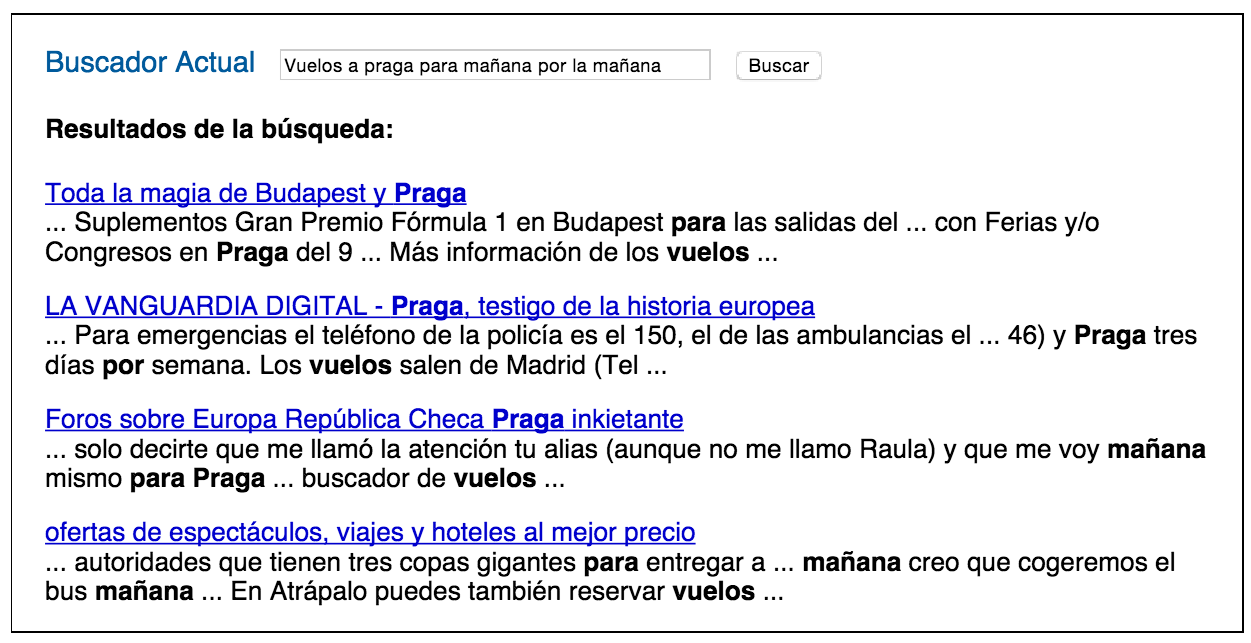
\includegraphics[width=400pt]{imgs/resultadoNormal}
\caption{Resultados obtenidos con un buscador normal.}
\end{center}
\end{figure}
\begin{figure}[H] %[h] Aqui [b] para button [t] para top
\begin{center}
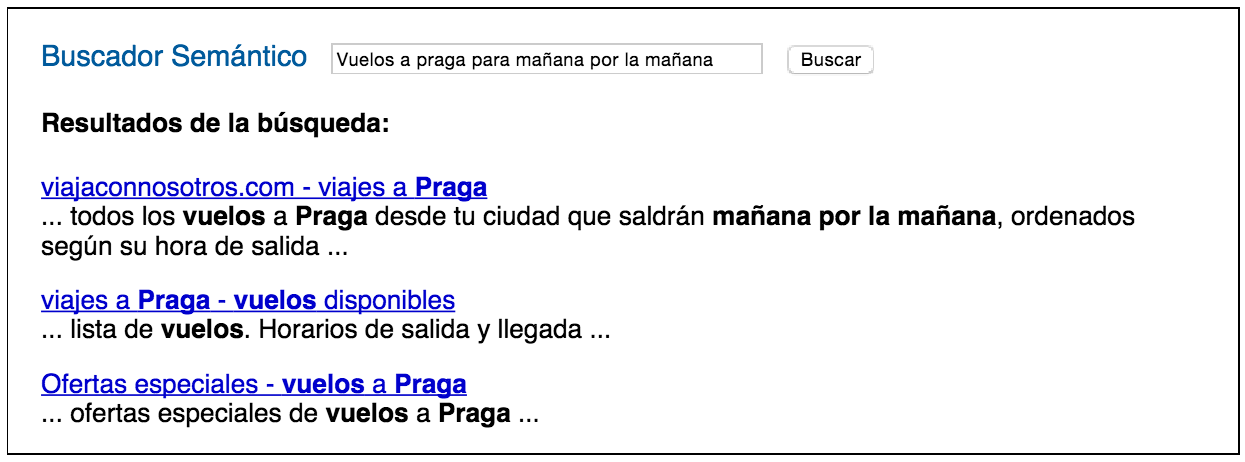
\includegraphics[width=400pt]{imgs/resultadoSemantico}
\caption{Resultados obtenidos con un buscador semántico.}
\end{center}
\end{figure}

\section{Resource Description Framework}
Es el principal formato de los datos de la Web Semántica. Un set de datos \textit{Resource Description Framework} (o \textit{RDF}) consiste en datos explícitos e implícitos presentes en la base de datos, dados por restricciones semánticas. Éstos son obtenidos por un proceso que considera todas las restricciones para inferir las posibles consecuencias de la base de datos existente.

Principalmente, proporcionan información descriptiva simple sobre los recursos que se encuentran en la Web y que se utiliza, por ejemplo, en catálogos de libros, directorios, colecciones personales de música, fotos, eventos, etc.\\

\textbf{Ejemplo:}\\
\newline
El texto: \textit{``Javier Perez es el autor del documento cuya URL es http://www.dc.uba.ar/examen.pdf. Su mail es jperez@dc.uba.ar y su teléfono +54(11)4563-4567.''} se representa de la siguiente forma:
\begin{verbatim}
<?namespace href="http://dc.uba.ar/info-bibliografia" as="bib"?> 
<RDF:serialization> 
  <RDF:assertions href="http://dc.uba.ar/examen.pdf"> 
    <bib:autor> 
      <RDF:resource> 
        <bib:nombre>Javier Perez</bib:nombre> 
        <bib:mail>jperez@dc.uba.ar</bib:mail> 
        <bib:telefono>+54(11)4563-4567</bib:telefono> 
      </RDF:resource> 
    </bib:autor> 
  </RDF:assertions> 
</RDF:serialization>
\end{verbatim}

\begin{center}
\begin{figure}[H] %[h] Aqui [b] para button [t] para top
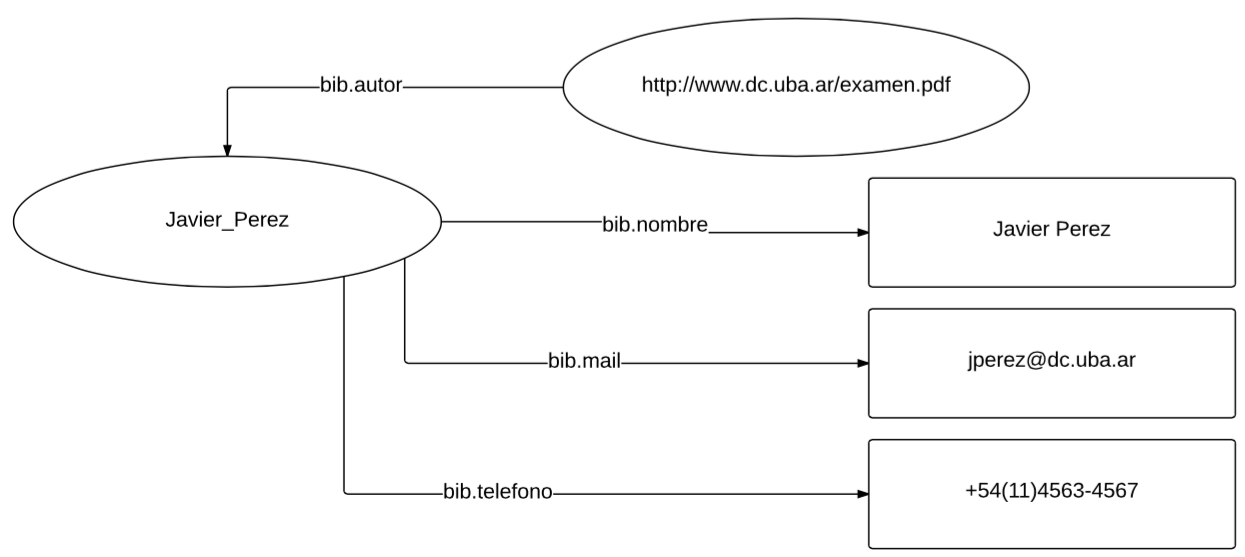
\includegraphics[width=400pt]{./imgs/rdfModel.png}
\caption{Modelo RDF.}
\end{figure}
Los nodos son las elipses, los ejes la relación y los rectángulos son strings.
\end{center}

\section{Problemas de la Web Semántica}
En el último tiempo, el uso de Web Semántica creció enormemente e impulsó la necesidad de emplear técnicas eficientes y escalables para responder a las consultas sobre una gran cantidad de datos heterogéneos. Una posible solución a este problema consiste en traducir las consultas \textit{RDF} en consultas \textit{SQL} para ejecutarlas en los sistemas de gestión de bases de datos relacionales (RDBMS), otra es hacer todos los datos implícitos. Sin embargo, las bases de datos para Web Semántica complican a las tecnologías clásicas de gestión de datos que no tienen en cuenta los datos implícitos durante la evaluación de consultas. Una solución a esto es reformular la consulta entrante para luego traducirla en una consulta SQL que, al ser evaluada por el RDBMS, devuelve las respuestas completas. El problema de esto es que no se logra un buen rendimiento debido a la longitud sintáctica de las consultas SQL que resultan de reformulación. Los RDBMs no son capaces de optimizar eficientemente las consultas, por lo que en algunos casos fallan o registran tiempos elevados de evaluación.

\section{RDF pasada a bases de datos tradicionales}
Las consultas RDF se pueden transformar en consultas de bases de datos relacionales sin mucha dificultad. A partir de la consulta transformada, es posible utilizar cualquiera de los dos métodos de vinculación de RDF para resolverla: saturación o reformulación.
\\\\
\textbf{Saturación:} Transforma los datos implícitos en explícitos, ampliando así la base de datos. 
\\\\
\textbf{Reformulación:} Se reformula la consulta basándose en las restricciones conocidas antes de evaluarla. La ventaja principal es que se aplica por consulta y no a toda la base de datos.

\section{Reformulación}

Como mencionamos anteriormente, las bases de datos para Web Semántica presentan datos implícitos que las RDBMs no tienen en cuenta a la hora de resolver las consultas. Para esto, se aplican técnicas de \textbf{Reformulación} a la consulta entrante para luego traducirla a una consulta SQL que, al ser evaluada por el Sistema de gestión de bases de datos relacionales, devuelve la respuesta completa. El problema de la reformulación es que puede presentar grandes problemas de rendimiento debido a la longitud sintáctica de las consultas SQL resultantes, como también generar fallas.

Existen distintas heurísticas que buscan solucionar los problemas de eficiencia. En su análisis, \textit{Damián A. Bursztyn} presenta dos de ellas.

En primer lugar, explica cómo obtener un espectro de consultas equivalentes obtenidas mediante el agrupamiento de fragmentos de la consulta original y la reformulación de los mismos. Estos fragmentos son enviados individualmente al RDBMs para su evaluación y unidos al momento de obtener los resultados.

Por otro lado, utiliza las distintas alternativas sintácticas propuestas por SQL para expresar el mismo tipo de consultas para estudiar qué elección es la más adecuada para mejorar el rendimiento. Para esto, realiza un análisis de las subconsultas provistas por el principal lenguaje informático de bases de datos relacionales.

\section{Conclusión}
Finalmente, podemos concluir que, más allá de la creciente popularidad de la Web Semántica, la resolución de las consultas RDF sigue presentando inconvenientes. La reformulación de RDF a SQL parece una buena solución, pero cuando el tamaño de la consulta resultante es demasiado grande aparecen problemas de eficiencia que pueden conducir a fallas. 

Si bien el problema de la Optimización de Consultas RDF reformuladas se investiga habitualmente, las únicas soluciones obtenidas hasta el momento no son más que heurísticas, que logran mejorar la eficiencia pero pueden fracasar en algunos casos.

\section{Referencias}

\begin{itemize}
\item The World Wide Web Consortium (W3C). http://www.w3c.es/Divulgacion/GuiasBreves/WebSemantica
\item W3C Recommendation. http://www.w3.org/TR/rdf-sparql-query/
\end{itemize}

\end{document}